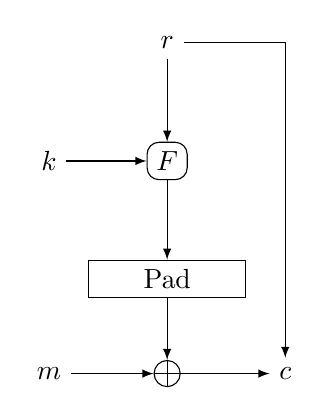
\begin{tikzpicture}
\node (r) {$r$};
\node (pg) [draw, below of = r, rounded corners=1ex,node distance = 1.5cm] {$F$};
\node (k) [left of = pg, node distance = 1.5cm] {$k$};
\node (pad) [minimum width=2cm, draw, shape = rectangle, below of = pg, node distance = 1.5cm] {Pad};
\node (xor) [below of = pad, circle, node distance = 1.2cm, draw] {};
\draw[-] (xor.north) -- (xor.south);
\draw[-] (xor.east) -- (xor.west);
\node (pt) [left of = xor, node distance = 1.5cm] {$m$};
\node (ct) [right of = xor, node distance = 1.5cm] {$c$};
\draw[-latex] (r) -- (pg);
\draw[-latex] (pg) -- (pad);
\draw[-latex] (pad) -- (xor);
\draw[-latex] (pt) -- (xor);
\draw[-latex] (xor) -- (ct);
\draw[-latex] (r) -| (ct);
\draw[-latex] (k) -- (pg);
\end{tikzpicture}